\documentclass[12pt,onecolumn]{article}
\usepackage{graphicx}
\usepackage{titletoc} 
\usepackage[english]{babel}
\usepackage{amsmath}
\usepackage{color}
\usepackage{float}
\setlength{\parindent}{0pt}
\usepackage[T1]{fontenc}
\usepackage{fancyhdr}   
\usepackage[a4paper,pdftex]{geometry}	
\usepackage{xcolor} 
\usepackage{enumerate}
\usepackage{fix-cm} 
\usepackage[notlof]{tocbibind}
\usepackage{amsmath}
\usepackage{listings}



\geometry{left=2.3cm,right=2.3cm,top=2.6cm,bottom=2.7cm}
\linespread{1.2}


\definecolor{codegreen}{rgb}{0,0.6,0}
\definecolor{codegray}{rgb}{0.5,0.5,0.5}
\definecolor{codepurple}{rgb}{0.58,0,0.82}
\definecolor{backcolour}{rgb}{0.95,0.95,0.92}
\definecolor{codeone}{rgb}{0.51,0.55,0.27}

\lstset{
	frame=tb,
	language=C,
	breaklines = true,
	backgroundcolor=\color{backcolour},   
	commentstyle=\color{gray},
	keywordstyle= \color{codeone},
	%\color{magenta},
	numberstyle=\tiny\color{codegray},
	stringstyle=\color{codepurple},
	basicstyle=\footnotesize,
	breakatwhitespace=false,         
	breaklines=true,                 
	captionpos=b,                    
	keepspaces=true,                 
	numbers=left,                    
	numbersep=5pt,                  
	showspaces=false,                
	showstringspaces=false,
	showtabs=false,                  
	tabsize=2
}





\begin{document}
\begin{titlepage}
\begin{center}

\includegraphics[scale=1.5]{CoverSheet}\\
\bf{ DEPARTMENT OF ELECTRICAL AND ELECTRONIC ENGINEERING }
\end{center}
\vspace{18mm}
 \begin{center}
 \begin{Large}
 \vspace{2.0cm}
 \bf{EEE212 Smart Refrigerator Lab Report}
 \end{Large}
 \end{center} 
\vspace{2.0cm}
  \begin{center}
  \begin{large}
     \begin{tabular}{l l} 
       Student Name & Strudnet ID\\ 
       \hline
       Ali Khan & 1406769\\
       Lingxuan Kong & 1405867\\ 
       Rishabh Aggarwal & 1407014\\
       Shiyao Zhang & 1405896\\
       Yuhao Wang & 1405404\\
       Zuopeng Liu & 1406090
       
    \end{tabular}
  \end{large}
  \end{center}
\clearpage
\end{titlepage}


\abstract{The following document reports our smart mini-refrigerator project, from planning the design to the final result. It explains some of the results and observations that were made as we progressed through the project, while also discussing the strengths and weakness of our product. The report also provides insight into how the fridge actually works. Our aim was to build a mini-refrigerator, that would serve as a suitable model for another project at a larger scale. Automatic temperature control as added to fridge using a relay. The mini-fridge was built within a week, but the design and planing consumed more time. In the end, the result was a satisfactory final product. The cooling was good, however the fridge itself had many weaknesses. }

\newpage
\tableofcontents

\newpage
\section{Introduction}
Home appliances have become a necessary part of our lives, providing comfort and luxury. A refrigerator is one such appliance that is crucial in one's household, rarely powered off. It is an engineering feat, which combines multiple engineering fields under one. The hardware and electronics are in perfect sync with each other providing cooling. This is the main reason that we chose to build a mini-refrigerator for this project. Our aim was to build a small fridge, one that could cool 3-4 cans of drinks. It would require no manual temperature control, i.e. the cooling inside the fridge was automatically controlled when the temperature dropped too low and vice versa. The report that follows describes how the project was approached, progressed and finally completed, with results and observations explained. It would attempt to become a guide to those who would want to build this mini-fridge. 

\section{Background Methodology}
\subsection{Peltier Effect}
The Peltier effect can be described as the temperature difference created when voltage is applied between two pieces of electrodes or conductors, which are directly connected to a semiconductor. It is also called the Thermoelectric effect, as a thermoelectric device is used to create a voltage difference in most cases. The Peltier effect allows heat or cold to be transferred from one medium to the other, utilizing the current flow between the two conductors. The figure below illustrates the Seebeck Circuit, which is used in cooling applications such as refrigerators. 

\begin{figure}[H]
	\centering
	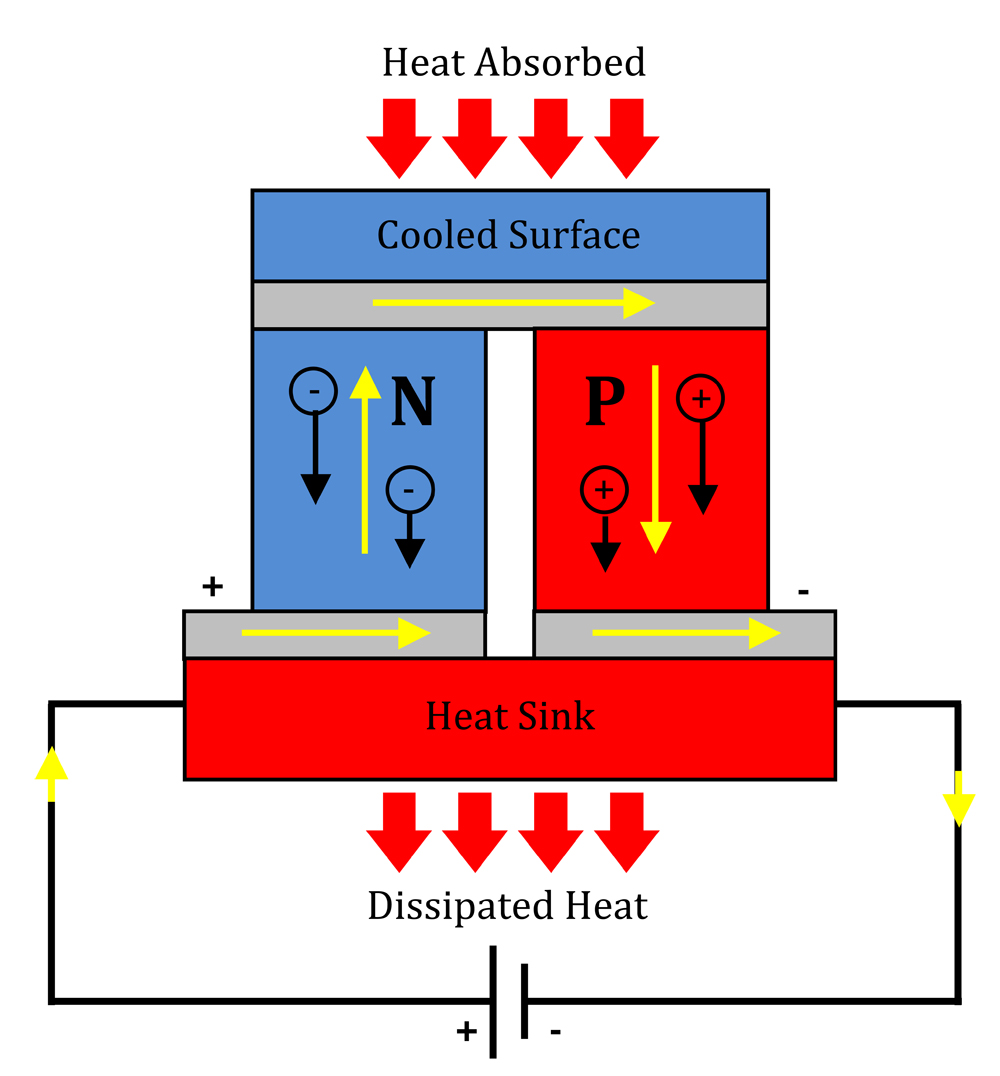
\includegraphics[scale=1.4]{peltier_effect}
	\caption{The Seebeck circuit as the peltier cooler}
\end{figure}


\subsection{Relay}
A relay is an electrically operated switch, switch on/off
mechanically using electromagnets.\\
Relays are used where it is necessary to control a circuit by a specific
low-power signal. For our project, we used a Magnetic Latching Relay
with a single coil. The relay operates in one direction when power is
applied with one polarity, and will reset when polarity is reversed.
\begin{figure}[H]
\centering
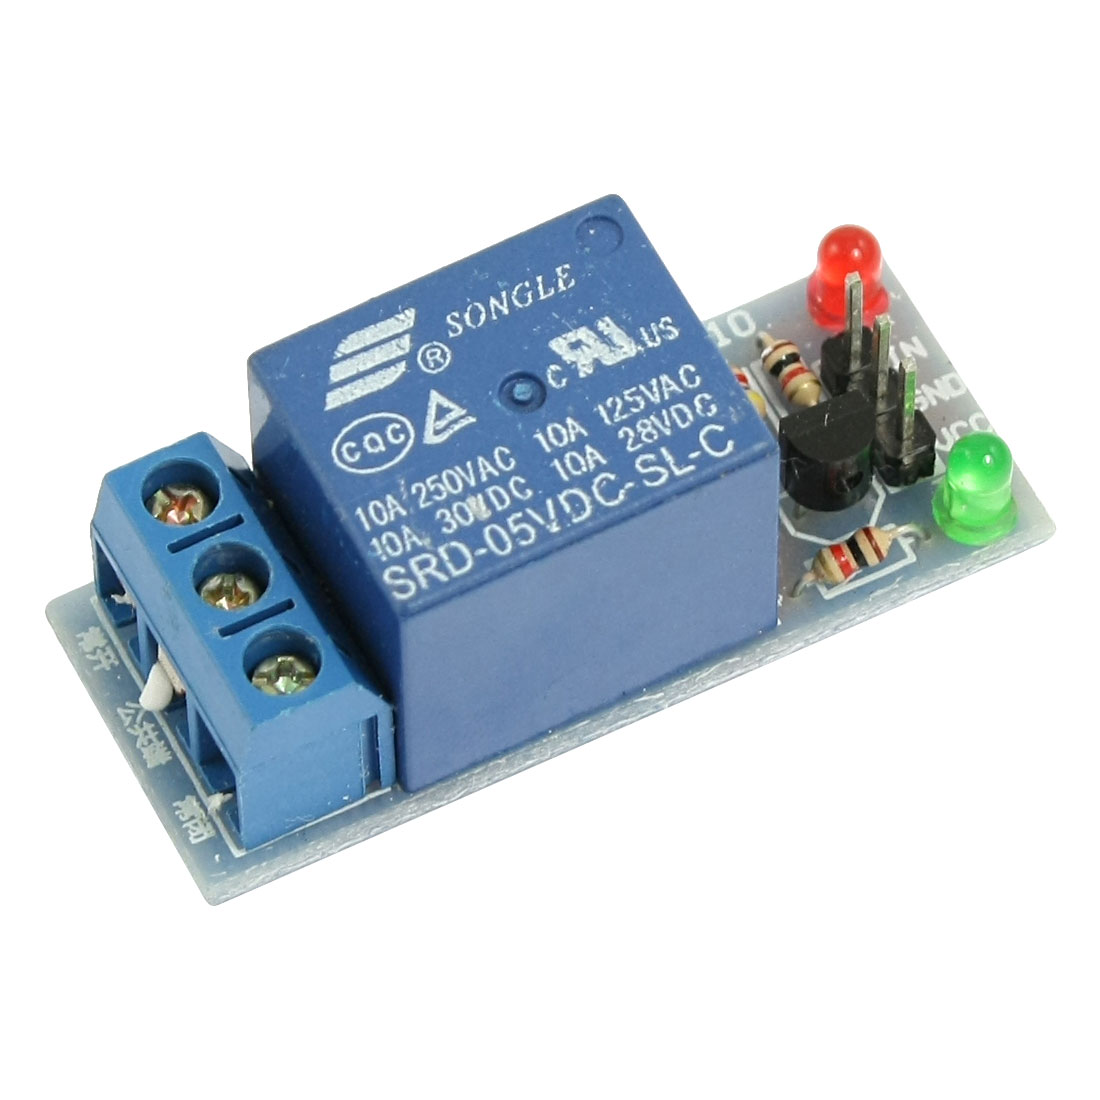
\includegraphics[width=3cm]{relay}
\caption{Magnetic Latching Relay}
\end{figure}

\subsection{Semiconductor}
According to the Peltier effect, we could used a semiconductor to build the cooling system in this refrigerator. The efficiency of the amount of cold on a semiconductor depends on the energy differential of two materials in charge carrier motion, which is also called thermoelectric difference. It is known that pure metal has good thermal conductivity but a low refrigeration efficiency. However, semiconductor materials have very high thermoelectric potential, which could be used in a small thermoelectric refrigerator.\\
According to the knowledge learned in EEE211, P-type semiconductor and N-type semiconductor has the maximum thermoelectric difference.\\
The figure 1 illustrates the semiconductor in the seebeck circuit, as a part of the peltier effect. According to this figure, we find that the P-pole has holes with positive charge and N-pole has electrons with negative charge. When these charges and holes moving in the P-N junction, there will be a potential difference between two poles creating a current. 
As the following picture shows, this is the semiconductor that we used:
\begin{figure}[H]
\centering
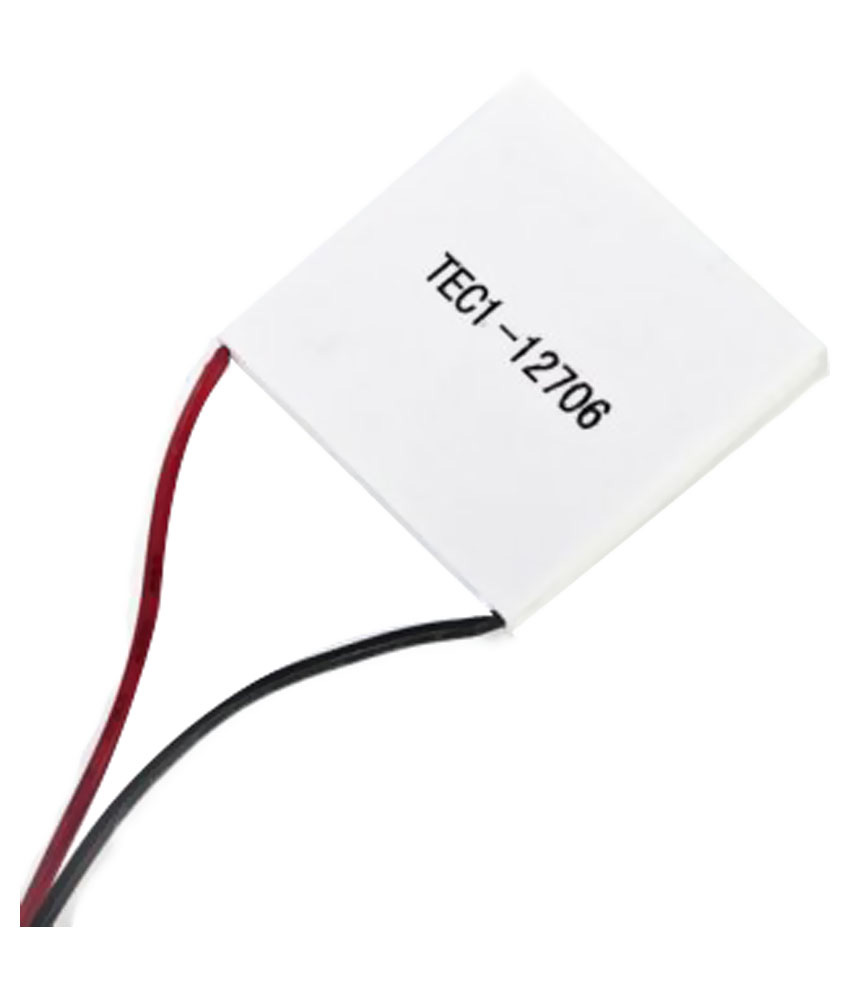
\includegraphics[width=6cm]{semiconductor}
\caption{The semiconductor}
\end{figure}

\subsection{Item List}
Following is the equipment used in building the refrigerator:
\begin{itemize}
	\item 12V 10A Thermoelectric Cooler
	\item Magnetic Latching Relay module
	\item Arduino Nano
	\item Temperature Sensor
	\item 12V 10A power supply
	\item Perforated Board
	\item Soldering Equipment
	\item Foam boards
	\item Hinges
	\item Plexiglass Panels
	\item Hot Glue-gun
	\item Pro's Kit Mini-drill
\end{itemize}

\begin{figure}[H]
	\begin{minipage}[t]{0.45\linewidth}
		\centering
		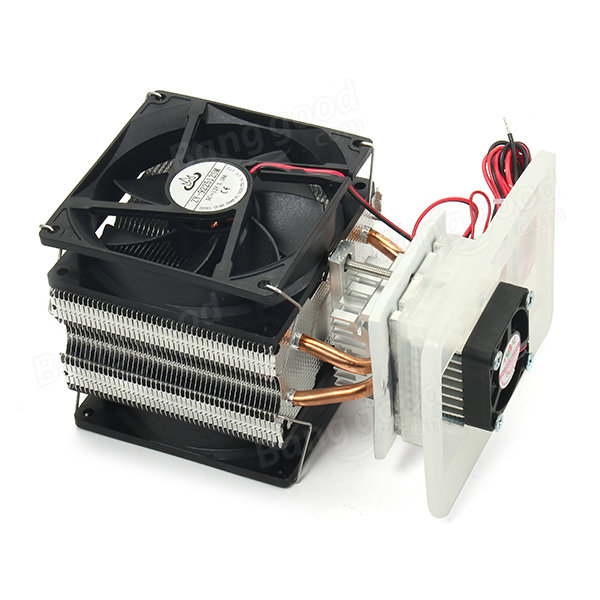
\includegraphics[width=4cm]{thermo_cooler}
		\caption{Thermoelectric Cooler}
	\end{minipage}%
	\hfill
	\begin{minipage}[t]{0.5\linewidth}
		\centering
		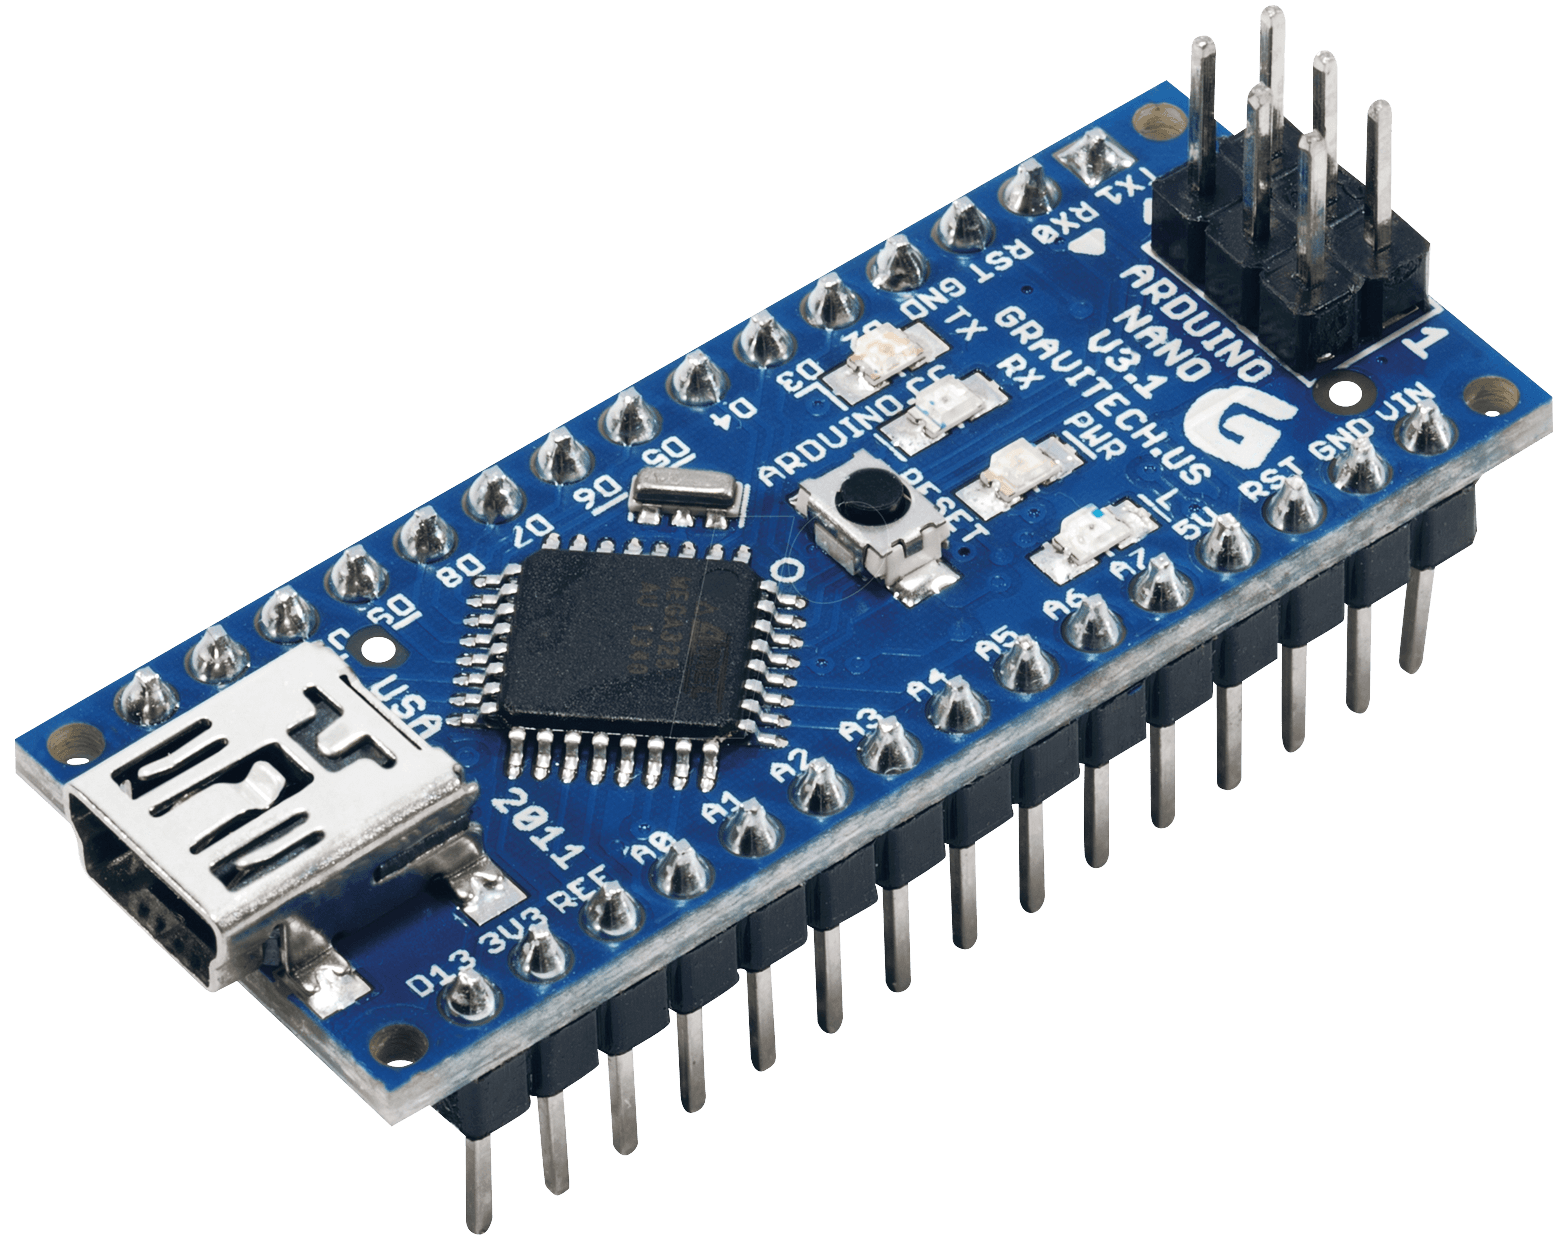
\includegraphics[width=4cm]{arduino_nano}
		\caption{arduino}
	\end{minipage}
\end{figure}

\begin{figure}[H]
	\begin{minipage}[t]{0.45\linewidth}
		\centering
		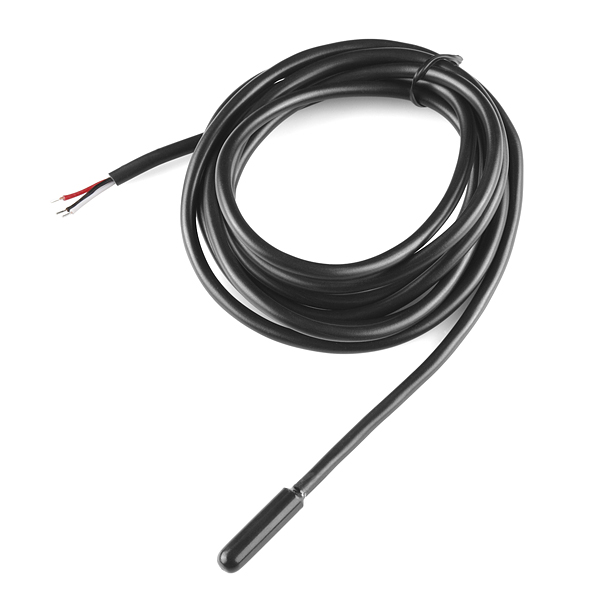
\includegraphics[width=4cm]{sensor}
		\caption{sensor}
	\end{minipage}%
	\hfill
	
\end{figure}

\subsection{Circuit Schematic}
\begin{figure}[H]
	\centering
	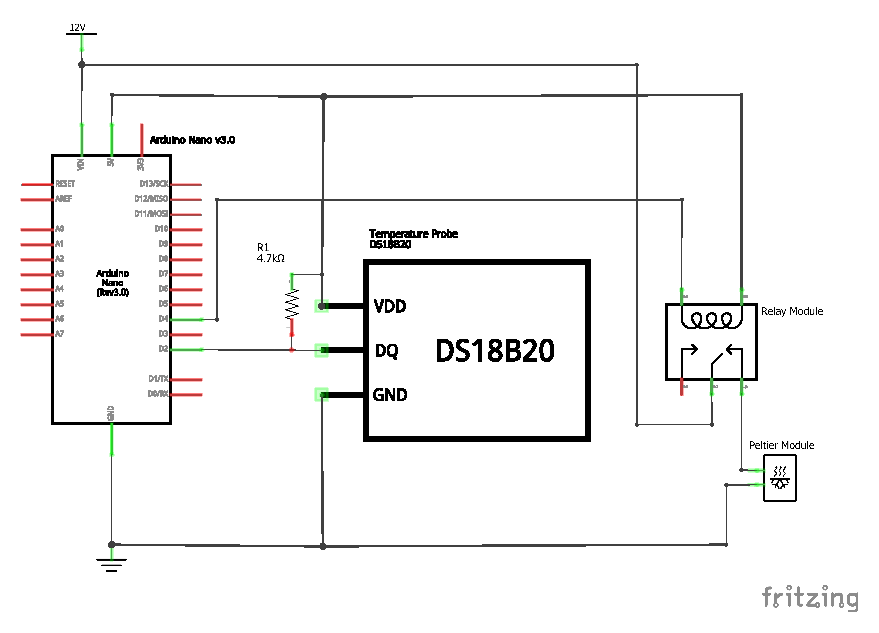
\includegraphics[scale=1.0]{mini_fridge_schem}
	\caption{Circuit Schematic of our control circuit}
\end{figure}
The circuit is designed to react towards the temperature change. The peltier module is controlled by a relay, which receives output data from digital port 4 on Arduino nano board, on the power supply chain. A temperature sensor, which detects the current temperature, is connected to digital port 2 on Arduino. Both Arduino and Peltier module are powered by a 12 volt supply while the temperature sensor and relay are powered by the 5 volt power supply of nano board. Theoretically, the relay module would switch its status according to the read of temperature sensor, powering the peltier module on or off. 

\subsection{Code}
The arduino code used in this project is listed in the Appendices.\\
When programming the arduino board, port number and temperature range were set where the temperature sensor is on port 2, the relay module is on port 4, and the ideal temperature range was selected between $3^{\circ}C$ and $7^{\circ}C$. The setup method initializes the sensor, pin mode, and initial output value. Read by sensor continuously in loop method, the current temperature would be compared with the temperature range set. The relay module would be turned off if current temperature is higher, and it would be turned on if current temperature is lower.



\section{Procedure}
The following procedure was followed when assembling the refrigerator. 
\begin{itemize}\itemsep -2pt
	\item In order to build the refrigerator, plexiglass panels were used. The reason is it is cheaper than other materials and temperature insensitive. The panels were cut and assembled using hot-glue gun. The whole box was split into 2 compartments, back one accomandating equipments, while the front compartment would act as the fridge.
	\item Foam boards were glued inside the refrigerator when box was completed. This would provide insulation, trapping the cool air. 
	\item The thermoelectric cooler was then placed in between the back and the front compartment. 
	\item The Arduino circuit was then assembled using the circuit schematic explained previously. 
	\item After testing the circuit was functional, the doors were attached to the front of the fridge. The back compartment was kept open, exposed to air, to maintain air flow. The hot air from the cooler was able to escape easily. 
\end{itemize}
The above steps are very brief because the assembly steps change depending on the design of the refrigerator. In our case, the mini-fridge only had the basic features, but adding other features like LED lighting would alter the circuit and assembly of the fridge.  

\section{Results}
After assembling the refrigerator, we measured the temperature to calculate the cooling efficiency. If it could not decrease the temperature below $10^{\circ}C$. It means that we should improve the cooling efficiency.\\  
The temperature values of the peltier module were measured before the it was assembled into the fridge and after assembly. This was to ensure that the temperature would go low enough to cool the fridge, while testing its efficiency. 

\subsection{Peltier Module minimum temperature recorded before assembly: $−6^{\circ}C$}
Using a portable temperature sensor, the temperature recorded was –6 degrees, and ice was observed on the cooling metal part. It was also observed that the temperature would drop more, but the drop was inconsistent and slow. Moreover, in this situation there was no fan attached to the cooling side.

\subsection{Peltier Module minimum temperature recorded after assembly:$-0.5^{\circ}C$} 
In this case the temperature recorded was $-0.5^{\circ}C$. This was with the fan attached so that there is air flow inside the fridge. The temperature was just low enough to provide cooling inside the volume of the fridge. However, the actual air temperature inside the fridge was just around $8^{\circ}C$, which is only acceptable. \\
After completing assembly of the mini-fridge, trials were conducted, each for 20-30 minutes, to check the cooling. The cooling of the fridge was found to be just satisfactory. \\
This refrigerator can be used in dormitories, so the temperature range was set between 3 degree and 7 degree, where the maximum is $7^{\circ}C$ and minimum is $3^{\circ}C$. At $3^{\circ}C$, the peltier module is powered off, while the fans are still on. Moreover, the fans are never turned off in order to maintain air flow through the cooler and the fridge. Turning the fans off may cause meling and rapid increase in temperature on the hotter side. 

\section{Strengths and weakness}
\subsection{Strength}
\subsubsection{Powerful Peltier Module Cooler}
The Peltier cooler includes a semiconductor which generates cooling by heat transfer through Peltier effect. It is more simple, sustainable and cheap. The cooling part is only a semiconductor. It does not need a pipe system to freeze the medium. In that case, it is a simpler design, when compared to a compressor. It also powerful, but not as energy efficient. 
\subsubsection{Large volume}
The volume is large. It could hold a dozen cans of coke or six boxes of rice. It is good enough for a university dormitory use.  
\subsubsection{Smart}
It is controlled by an Adinuo broad. It adjusts the temperature automatically. No manual control is needed for temperature control. It is automatically controlled between set temperature range. 
\subsection{Weaknesses}
\subsubsection{Low cooling}
It takes about 5-10 minutes to make the inside cool and reach the lowest cooling. The cooling efficiency inside the fridge is low, mainly because the thermoelectric cooler is inefficient.
\subsubsection{Improper insulation}
The insulation is very important for a fridge. It strongly impacts the performance of the fridge. There are some gaps through the fridge to put the sensor in. In that case, cross-ventilation would occur, which makes the temperature increase very fast and decrease slow. It also makes the lowest temperature very high even if a 70-degree difference was caused when the cooling part is working. The body of the fridge is made up of foam broad which is relatively thin. It is a good insulation material but not good enough. Touching the body when the fridge working, it feels cool. That means the foam broad cannot prevent the heat exchange properly.
\subsubsection{Non-Portable}
The non-portable design makes the fridge hard to carry. Its not convenient to carry when traveling. The door has no handle which makes the fridge hard to open. Door handle was not attached as it was putting weight on the door, ripping the hinges apart. 
\subsubsection{Fragile}
It is made of thin plexiglass and stuck together by glue, so the overall fridge is fragile. Long term use may wear the glue down due to oxidation. 

\section{Problems}
\subsection{Choosing an appropriate power supply and cooler}
For powering this fridge, one rectifier which can convert 220V AC is needed. For better performance, the power supply should be maximized. However, two constrains, namely the circuit and cooler module's limited affordability, denied this straight scenario. \\
Firstly, it has been tested that the 1-mm-diameter wire can not stand current exceeding 3A. In the testing, the rubber wrapping the metal melts within one minute.\\ 
Secondly, the current-voltage rating of these two devices need to be compatible with each other. If rectifier's voltage is larger than peltier module's voltage rating, substance inside semiconductor might lose initial chemical property and may not work properly. 
\subsection{Select the suitable fluctuation range for temperature control}
As introduced before, the temperature range is set from $3^{\circ}C$to $7^{\circ}C$.  For better cooling performance, the lower temperatuer set should be as low as possible. However, the control function can not be activated unless this lower temperature can be ensured to be reached. Thus, this temperature has to be achievable but predicting the lowest achievable temperature is difficult because of the multiple factors affecting the performance. They test results varies from $0.5^{\circ}C$ the best one, to $2.1^{\circ}C$ the worst. According to this, the lower turn-point is set to $3^{\circ}C$ \\
On the other hand, the upper turn-point was chosen based on two targets. The first, to provide better demonstration of turn-on-off control. The second, to offer on interval time to enable cooler to dissipate heat on the hotter side.
\subsection{Selecting insulating material}
Insulation is one vital feature for performance of fridge. At the beginning, styrene foam board was considered for its convient utility. However, this material is too thick to be portable and extremely fragile. Additionally, it is conceived to place one LED lighting inside the fridge initially, so this fridge chamber was planed to be transparent. As a result, plexiglass was chosen as the insulration material. 
\subsection{Deciding the volume of fridge}
This dilemma is one compromise between the cooling performance and the capacity. The lowest temperature can be literally improved by shrinking the space inside this fridge but it will hamper the practicality. One of the objective is to make the fridge applicable enough to be used in daily life, so the volume should be as large as possible on the promise that the cooling effect is satisfactory. \\
However, the resultant performance was unkowned before assemblying and testing. Consequently, it is extremely hard to predict the ideal volume. On the other hand, temperature will decrease constantly if the insulation is perfect no maetter how much the volume is. Finally, the volume was decided to be 15 liters. \\

\section{Improvements}
\subsection{LED lighting}
For demonstration of the cooling effect, one LED lighting, is planned to be placed in this fridge. The mechanism is that the internal resistance vary with temperature, i.e. the lower the temperature, the smaller the resistance. Thus, the luminance of LED will increase with decreasing temperature. Nevertheless, this plan is aborted for reasons including the limited visual effect, potential implication to fridge's operation, and difficulty of finding appropriate LED lighting. \\
Otherwise, it should be practical if suitable LEDs lighting is found. It is feasible if several LEDs beads of 1.5V or 3V voltage rating in series can be applied and configured. However, this would complicate the assembly of the whole fridge.
\subsection{Reduce the volume}
The tested result of the peltier module was $7^{\circ}C$ and anticipated fridge temperature is just below $0^{\circ}C$ However, the resultant temperature does not reach the anticipated value as mentioned before. The volume can be regarded as one contributor, thus should be reduced.
\subsection{More powerful cooler}
This improvement is straight and has been already done been taken into account once. The second 12V-10A power supply replaced the first one, whose specification is 5V-3A. Subsequently, the second peltier module has a larger power rating. The result of this improvement has been already confirmed. The results of lowest temperature test of peltier module exposure in environment are $-2^{\circ}C$and $-7^{\circ}C$respectively. Moreover, a set of more energetic power supply and peltier module can improve the performance further. 
\subsection{Better insulation}
To prevent external heat from transmitting into the fridge, there can be two scenarioes, besides better construction and adherence. \\
The first is to make the plexiglass and foam board thicker and the external heat will not intrude. However, this one will cost much because this adamantine plexiglass is expensive and hard to modify. It will also increase overall weight.\\
The second one is changing the insulating material. It is not practical to apply metal or other expensive material with internal vacuum. The best option is still chemical polymer. The cheap, light styrene foam board is one exceptional choice, at the expense of transparent visual effect.  




\section{Photo of the whole refrigerator}
\begin{figure}[H]
	\centering
	\includegraphics[width=11cm]{fridge1}
	\caption{The photo of fridge front}
\end{figure}

\begin{figure}[H]
	\centering
	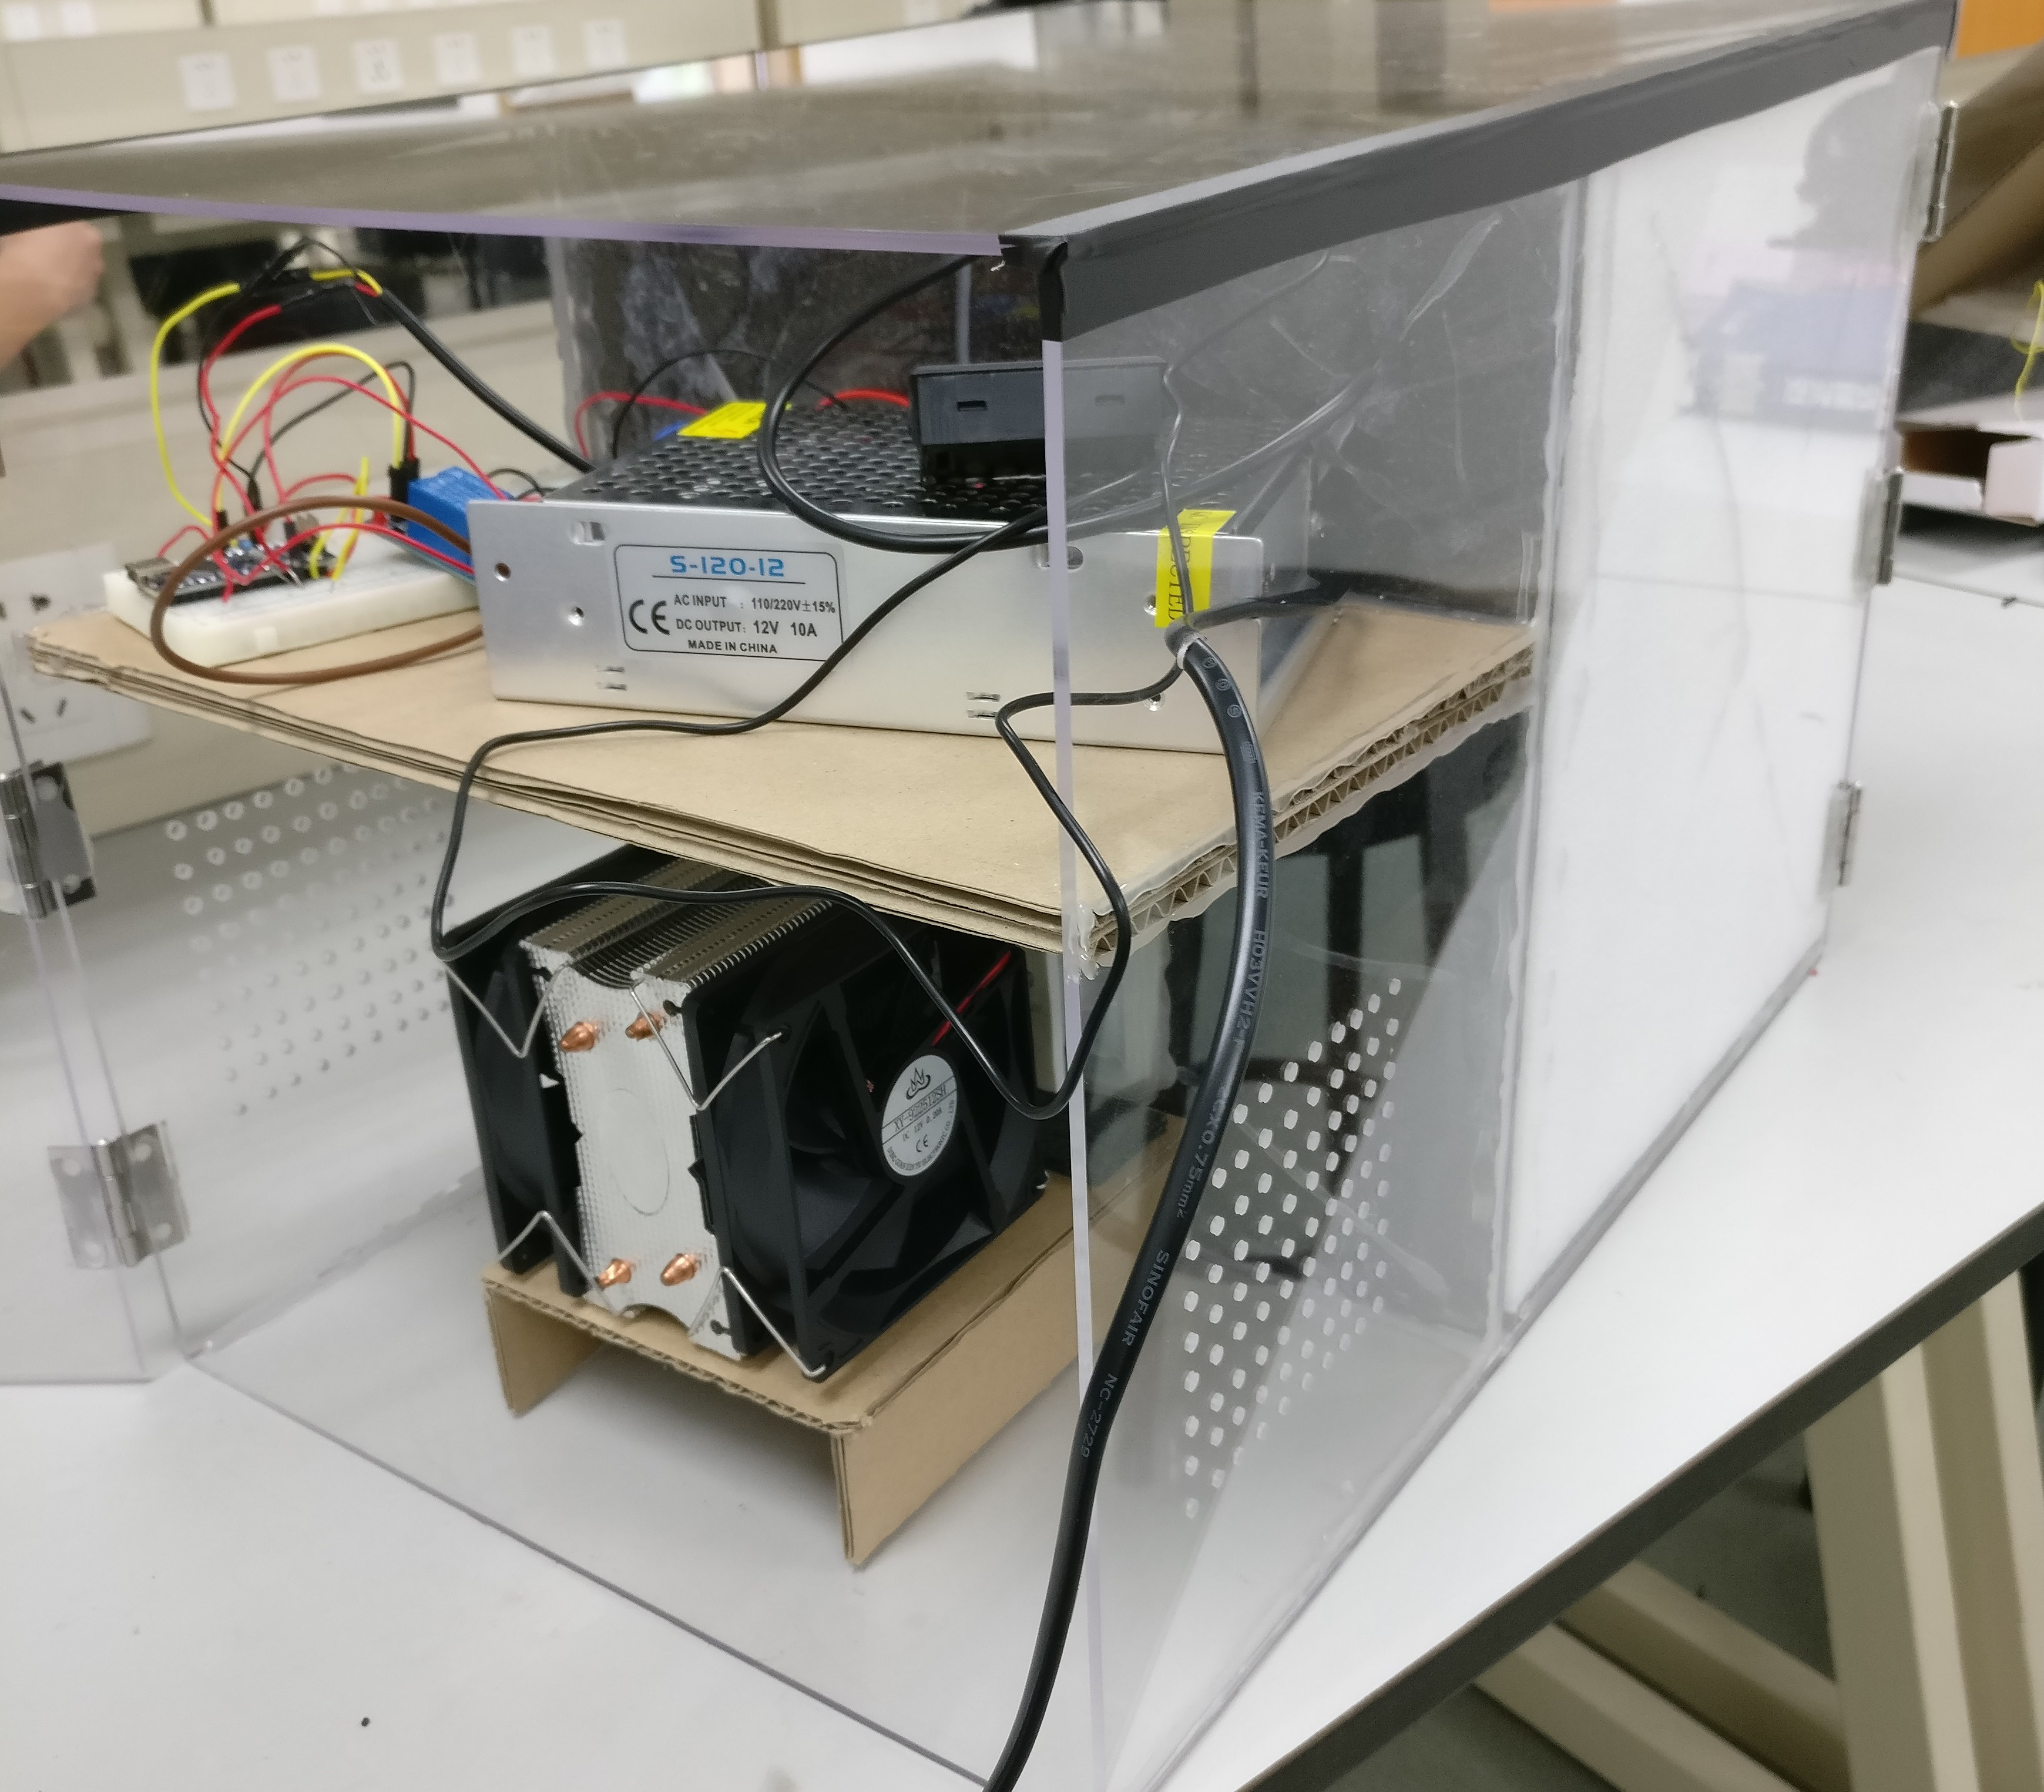
\includegraphics[width=11cm]{fridge2}
	\caption{The photo of fridge front back}
\end{figure}


\section{Conclusion}
The aim of the project was to build a mini-refrigerator that could cool three or four cans of drinks. The fridge must be controlled automatically, with manual touch. We used thermoelectric cooler, relay, Arduino, temperature sensor, and others to assemble the fridge. A simple feedback circuit with Arduino codes was implemented to control temperature inside. The assembled refrigerator could reach -0.5 Celsius. Our fridge is simple, powerful, and smart with a large amount of volume. However, it is inefficient, improperly insulated, non-portable, and fragile. Meanwhile, we have faced several problems including how to choose an appropriate power supply and cooler, how to choose a suitable range of temperature, and so on. As future expansion, we could: add LED lights, reduce volume for higher efficiency, use a more powerful cooler, and make the design more compact.
\newpage
\bibliographystyle{IEEEtran}
\nocite{*}
\bibliography{ref}
\newpage
\section{Appendices}
\lstinputlisting[language = C++]{F1VTS29IVO5D4XS.ino}

\end{document}
